\section{Surroundings}
  \includecpp{setup}{./Contest_Setup.txt}
  \includecpp{bashrc}{./Surroudings/.bashrc}
  \includecpp{vimrc}{./Surroudings/.vimrc}
\section{Data\_Structure}
  \includecpp{Sparse\ Table}{./Data_Structure/SparseTable.cpp}
  \includecpp{Fenwick\ Tree}{./Data_Structure/FenwickTree.cpp}
  \includecpp{單點修改、區間查詢線段樹}{./Data_Structure/SegmentTree2.cpp}
  \includecpp{最大區間和線段樹}{./Data_Structure/MaxSumSegmentTree.cpp}
  \includecpp{懶標線段樹}{./Data_Structure/LazyTagSegmentTree.cpp}
  \includecpp{持久化線段樹}{./Data_Structure/PersistentSegmentTree.cpp}
  \includecpp{李超線段樹}{./Data_Structure/LiChao.cpp}
  \includecpp{Treap}{./Data_Structure/Treap.cpp}
  \includecpp{Dynamic\_KD\_tree}{./Data_Structure/Dynamic_KD_tree.cpp}
  \includecpp{Heavy\ Light}{./Data_Structure/HeavyLight.cpp}
  \includecpp{HLD\ By\ Koying}{./Data_Structure/HLD_Koying.cpp}
  \includecpp{Link\ Cut\ Tree}{./Data_Structure/link_cut_tree.cpp}
\section{DP}
  \includecpp{LCIS}{./DP/LCIS.cpp}
  \includecpp{Bounded\_Knapsack}{./DP/Bounded_Knapsack.cpp}
  \includecpp{1D1D}{./DP/DP_1D1D.cpp}
\section{Graph}
  \includecpp{Dijkstra}{./Graph/Dijkstra.cpp}
  \includecpp{Bellman\ Ford}{./Graph/BellmanFord.cpp}
  \includecpp{SPFA}{./Graph/SPFA.cpp}
  \includecpp{Prim}{./Graph/Prim.cpp}
  \includecpp{Mahattan\ MST}{./Graph/MahattanMST.cpp}
  \includecpp{LCA}{./Graph/LCA.cpp}
  \includecpp{Tarjan}{./Graph/Tarjan.cpp}
  \includecpp{BCC\_edge}{./Graph/BCC_edge.cpp}
  \includecpp{最小平均環}{./Graph/MinMeanCycle.cpp}
  \includecpp{2-SAT}{./Graph/Two_SAT.cpp}
  \includecpp{生成樹數量}{./Graph/KirchhoffMatrixTree.cpp}
\section{Flow\_Matching}
  \includecpp{Dinic}{./Flow_Matching/Dinic.cpp}
  \includecpp{Min\ Cost\ Max\ Flow}{./Flow_Matching/Min_Cost_Max_Flow.cpp}
  \includecpp{Ford\ Fulkerson}{./Flow_Matching/Ford_Fulkerson.cpp}
  \includecpp{KM}{./Flow_Matching/KM.cpp}
  \includecpp{Hopcroft\ Karp}{./Flow_Matching/Hopcroft_Karp.cpp}
  \includecpp{SW-MinCut}{./Flow_Matching/SW_MinCut.cpp}
  \includecpp{Stable\ Marriage}{./Flow_Matching/Stable_Marriage.cpp}
\section{Math}
  \includecpp{快速羃}{./Math/FastPow.cpp}
  \includecpp{模逆元}{./Math/ModInv.cpp}
  \includecpp{離散根號}{./Math/Discrete_sqrt.cpp}
  \includecpp{外星模運算}{./Math/外星模運算.cpp}
  \includecpp{SG}{./Math/SG.cpp}
  \includecpp{Matrix}{./Math/Matrix.cpp}
  \includecpp{Karatsuba}{./Math/Karatsuba.cpp}
  \includecpp{Euler\ Function}{./Math/EulerFunction.cpp}
  \includecpp{Miller\ Rabin}{./Math/MillerRabin.cpp}
  \includecpp{質因數分解}{./Math/prime_factorization.cpp}
  \includecpp{質數}{./Math/PrimeList.cpp}
  \includecpp{實根}{./Math/FindRealRoot.cpp}
  \includecpp{FFT}{./Math/FFT.cpp}
  \includecpp{NTT}{./Math/NTT.cpp}
  \includecpp{Simplex}{./Math/Simplex.cpp}
  \includecpp{Expression}{./Math/Expression.cpp}
  \includecpp{Pick's Theorem}{./Math/Pick's_Theorem.cpp}
  \includecpp{擴展歐幾里德}{./Math/extgcd.cpp}
  \includecpp{線性篩}{./Math/線性篩.cpp}
\section{String}
  \includecpp{Rolling\ Hash}{./String/RollHash.cpp}
  \includecpp{Trie}{./String/Trie.cpp}
  \includecpp{AC自動機}{./String/AC自動機.cpp}
  \includecpp{KMP}{./String/Kmp.cpp}
  \includecpp{Z}{./String/Z.cpp}
  \includecpp{BWT}{./String/BWT.cpp}
  \includecpp{Suffix\_Array\_LCP}{./String/suffix_array_lcp.cpp}
  \includecpp{LPS}{./String/LPS.cpp}
  \includecpp{Edit\ Distance}{./String/Edit_Distance.cpp}
\section{Geometry}
  \includecpp{Geometry}{./Geometry/Geometry.cpp}
  \includecpp{旋轉卡尺}{./Geometry/旋轉卡尺.cpp}
  \includecpp{最近點對}{./Geometry/ClosestPair.cpp}
  \includecpp{最小覆蓋圓}{./Geometry/SmallestCircle.cpp}
  \includecpp{Rectangle\ Union\ Area}{./Geometry/Rectangle_Union_Area.cpp}
\section{Other}
  \includecpp{Fastio}{./Other/Fastio.cpp}
  \includecpp{pbds}{./Other/pbds.cpp}
  \includecpp{BuiltIn}{./Other/BuiltIn.cpp}
  \includecpp{莫隊算法-區間眾數}{./Other/莫隊算法_區間眾數.cpp}
  \includecpp{CNF}{./Other/CNF.cpp}
  \includecpp{提醒事項}{./Other/Reminder.cpp}
  \subsection{霍夫曼樹}
  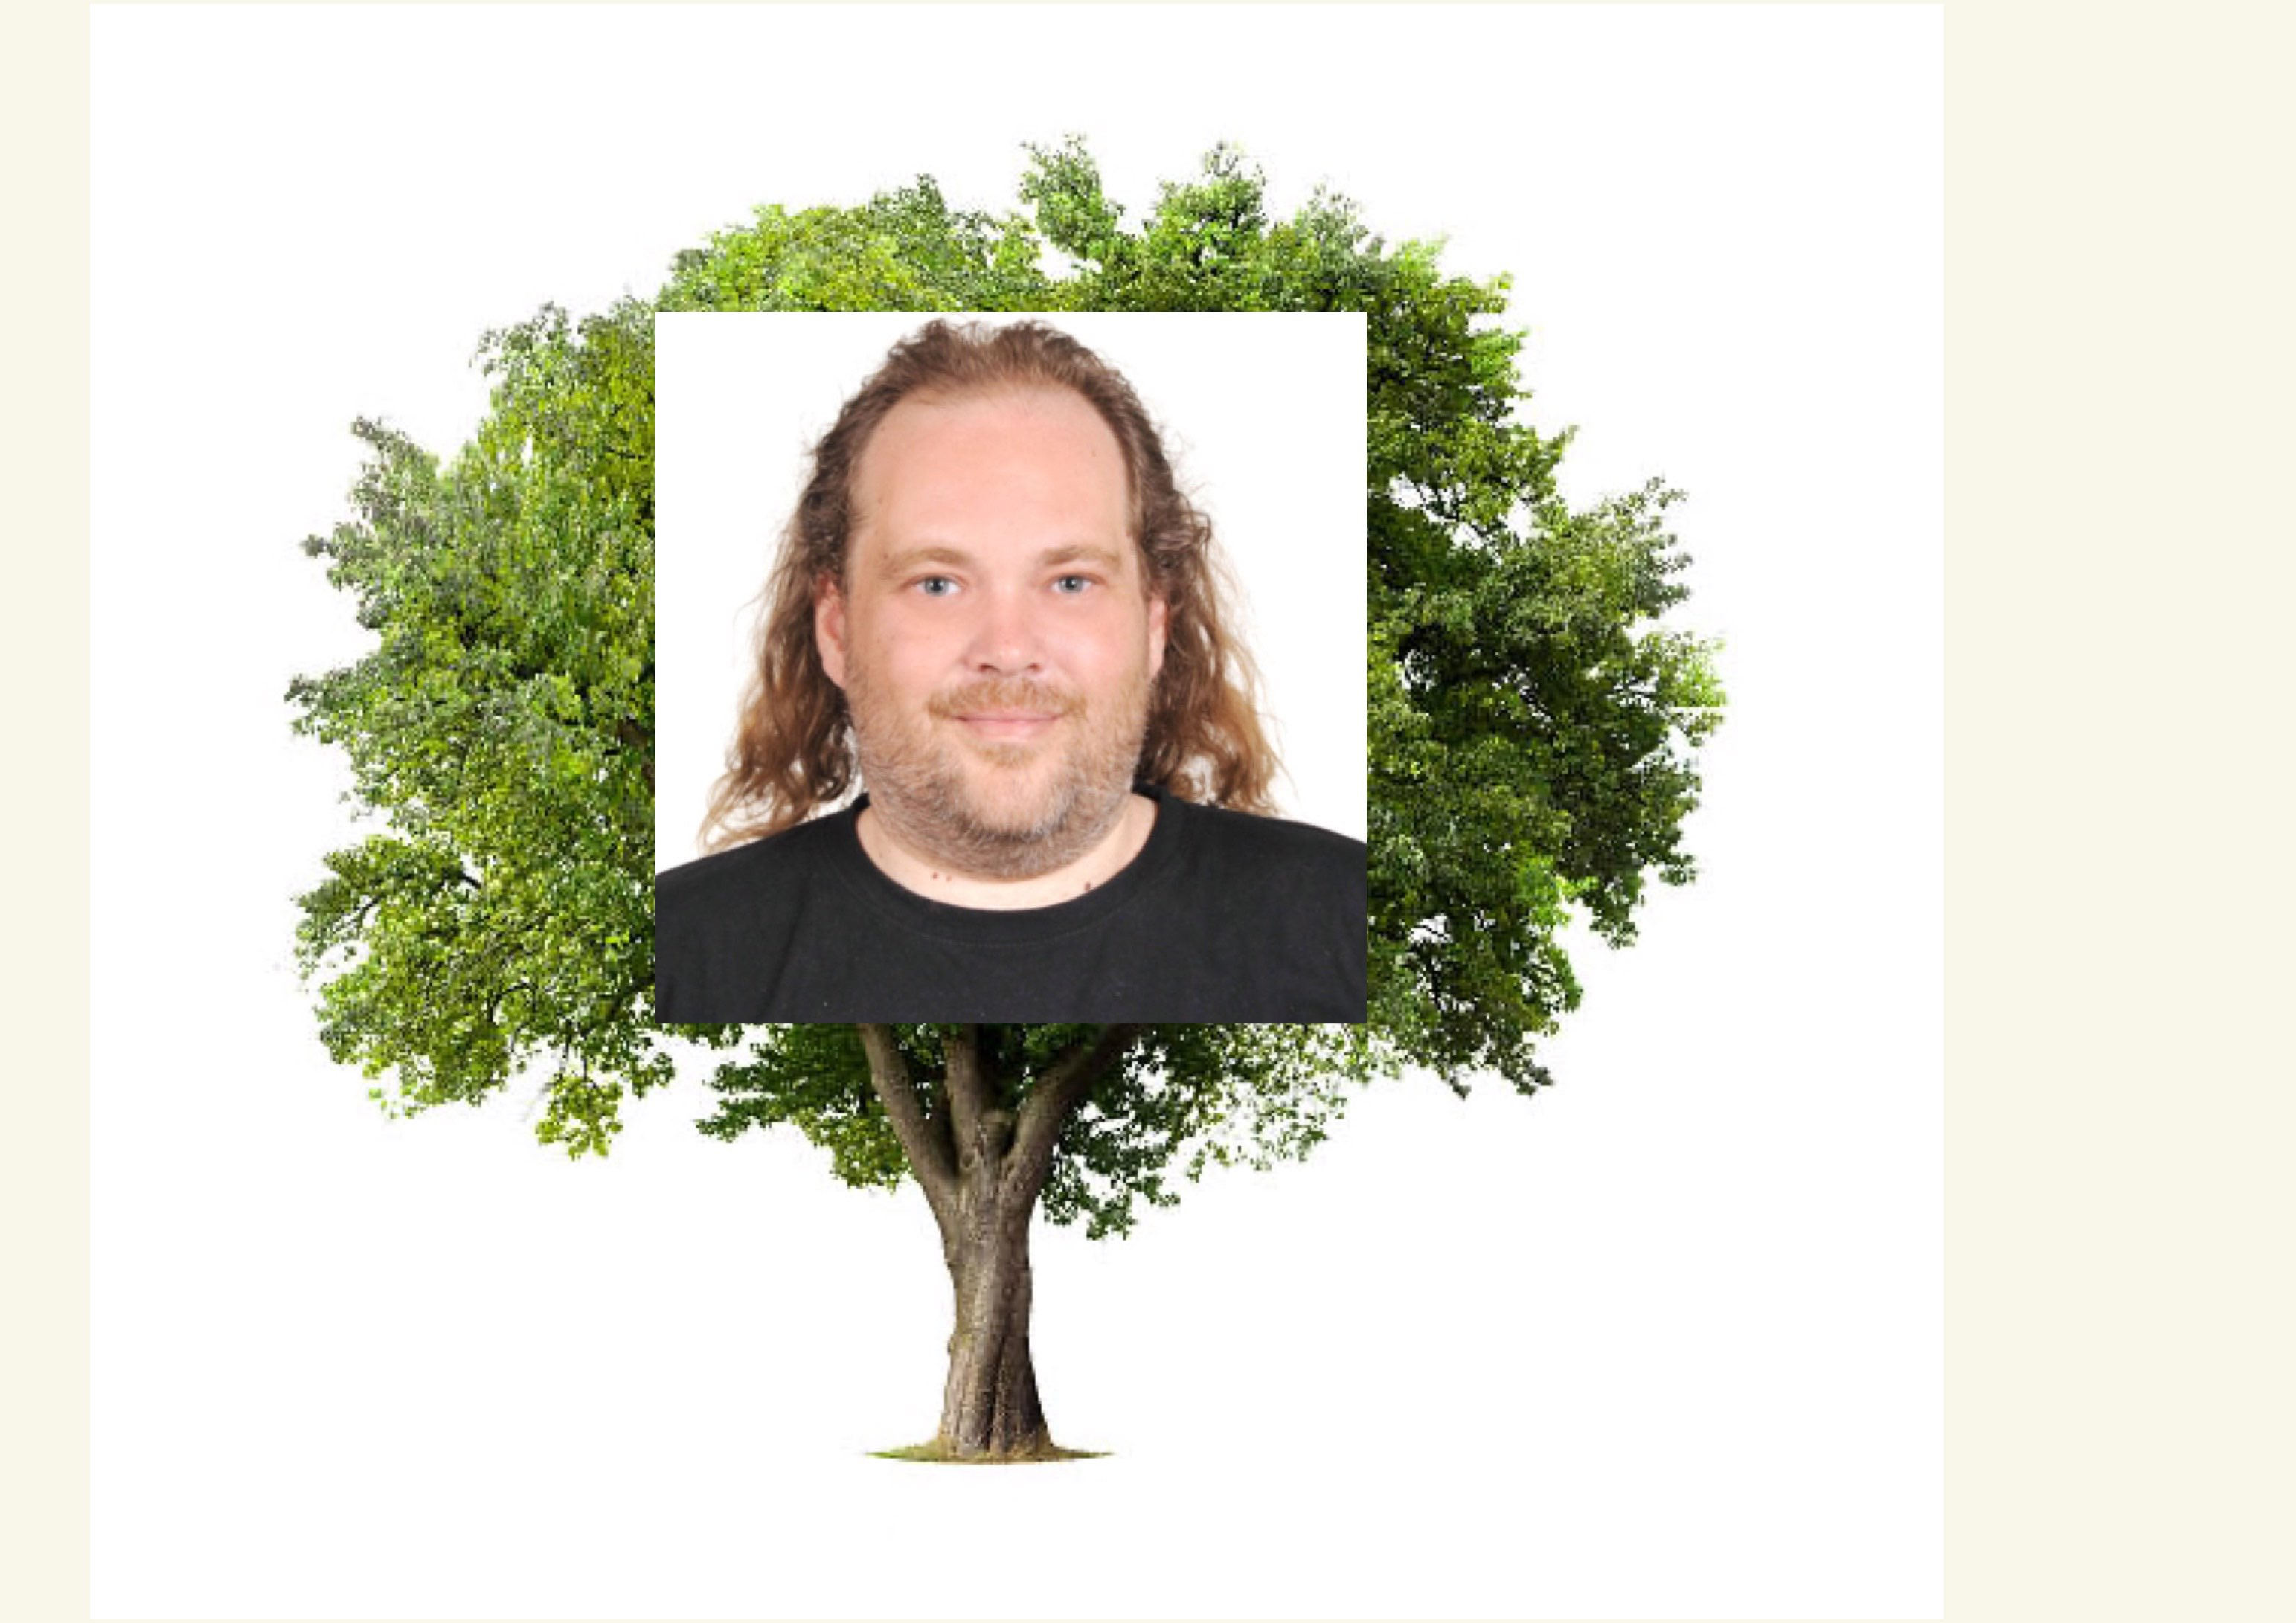
\includegraphics[width=0.25\textwidth]{霍夫曼樹.jpg}
